\scanpage{96}
% archive foliation: 95 No author page-number visible.
jouant un rôle universel pour \deleted{\unsure{ces}}\inserted{de telles} données
($\underline J$ torseur sous $(\mathbb Z/3\mathbb Z)_S$, $t\in\Gamma(\Sigma_{\underline J}^*/S)$,
$\omega\in\Gamma(S,\underline\omega_{\underline J})$
correspondant à la structure de torseur sur $\underline J$,
et donnant lieu à une trivialisation de
$\underline\omega_{\underline J}$ sur $S$\ldots). Les deux pts de
vue sont équivalents, quand on se fixe
une section $i$ de $\unsure{\boldsymbol{\mu}|\mu}_4^*$, i.e. quand on
travaille au dessus de la base $\widetilde S_0=\unsure{\boldsymbol{\mu}|\mu}_{4S_0}^*$
($S_0=\operatorname{Spec}\mathbb Z[\frac12]$).
\figure{\begin{tikzpicture}\draw (0,0)--(1,0);\end{tikzpicture}}
Explicitons entièrement la notion d'épinglage de
Legendre, du point de vue calculatoire, sur un
corps de base alg. clos $k$ pour simplifier, en
décrivant la courbe elliptique $E$ sur $k$ en termes
de
\figure{\begin{tikzpicture}[x=1cm,y=1cm]
\node[anchor=west] at (0,1) {$J(={}_2E(k)^*)$};
\node[anchor=west] at (3.1,1) {(ens. à trois éléments), du};
\node[anchor=west] at (-0.3,0) {$(58)\quad k$-vectoriel};
\node[anchor=west] at (3,0) {$V_J=\deleted{\unsure{k^J}}\operatorname{Ker}(k^J\xrightarrow{\mathrm{somme}}k)$};
\draw (-0.4,0.65)--(0,0.65)--(0,1.35)--(3.1,1.35)--(3.1,0.65)--(9.5,0.65)--(9.5,-0.1);
\draw (2.3,-0.3)--(3,-0.3)--(2.9,0.35);
\end{tikzpicture}}
(d'où
\[
(59)\qquad\Sigma_J=\operatorname{Proj}(V_J),\quad\text{avec }\deleted{\unsure{q}}\text{ des }\xi_i\in\Sigma_J(k)\ (i\in J)\quad\text{d'où}
\]
$\Sigma_J^*=\Sigma_J-\{\xi_i\}_{i\in J}$), et un $t\in\Sigma_J^*$ i.e. une
droite
\[
(60)\qquad F_t\subset V_J,
\]
% margin position: left, slanted
\margin{$\xi_i=\unsure{k.(e_j-e_k)}$ où $(e_i)$ est la base can. de $\unsure{V_J}$}
enfin un $k$-module inv. $\underline t_{\unsure{E}}$ \inserted{($=T_E$)} et un isom
\[
(61)\qquad \nu\,(=\nu_{\unsure{E}}):\underline t_{\unsure{E}}^{\otimes2}\simeq T_{\Sigma_J,t}.
\]
Il faut d'abord expliciter calculatoirement $T_{\Sigma_J,t}$
